\chapter{Suggestion}
In the chapter Suggestion the datasets are selected. Further, the procedure on how to set up the experiments is to be determinded.

\section{Selection of Datasets}
In order to find, which Neural Network architecture is better suited for anomaly detection, first, suitable datasets have to be evaluated. Most of the papers on anomaly detection test on one of the popular benchmark datasets such as the ones created by Numenta, Yahoo, NASA, or Pei's Lab. These benchmark datasets are, however, declared as flawed by Wu and Keogh \parencite{YEAR}. Wu and Keogh state that the benchmark datasets suffer at least one of the following flaws:

\begin{enumerate}
	\item Triviality: Surprisingly, a sizable proportion of the problems in the benchmark datasets are trivial to solve. Triviality is hereby defined as follows: An anomaly can be found with just one line of code.
	\item Unrealistic Density: This flaw refers to too many anomalies in the dataset or at least in a certain region, whereas in a real world dataset the anomalous data points make up a portion of just above 0 percent.   
	\item Mislabeled Ground Truth: The data in all of the benchmark datasets appears to be mislabeled, with both false positives and false negatives. This is significant for a number of reasons. The majority of anomaly detectors work by computing statistics for each subsequence of some length. They may, however, place their computed label at the beginning, end, or middle of the subsequence. If caution is not exercised, an algorithm may be penalized for reporting a positive just to the left or right of a labeled region.
	\item Run-to-failure Bias: Because many real-world systems are run-to-failure, there is often no data to the right of the last anomaly. Therefore, a naïve algorithm that labels the last point as an anomaly has a very good chance of being correct.
\end{enumerate}

In their work, Wu and Keogh, introduced the UCR Time Series Anomaly Datasets as new benchmark, that avoids the problems listed above. However, at the start of this research project the datasets were not publicly available. Because the search for a dataset, that does not suffer from the above mentioned flaws, would be too time-consuming, the decision was taken to engineer own datasets.\\
 \\
 

   

\section{Anomalies}
https://arxiv.org/ftp/arxiv/papers/2007/2007.15634.pdf

\begin{figure}[h]
	\centering
	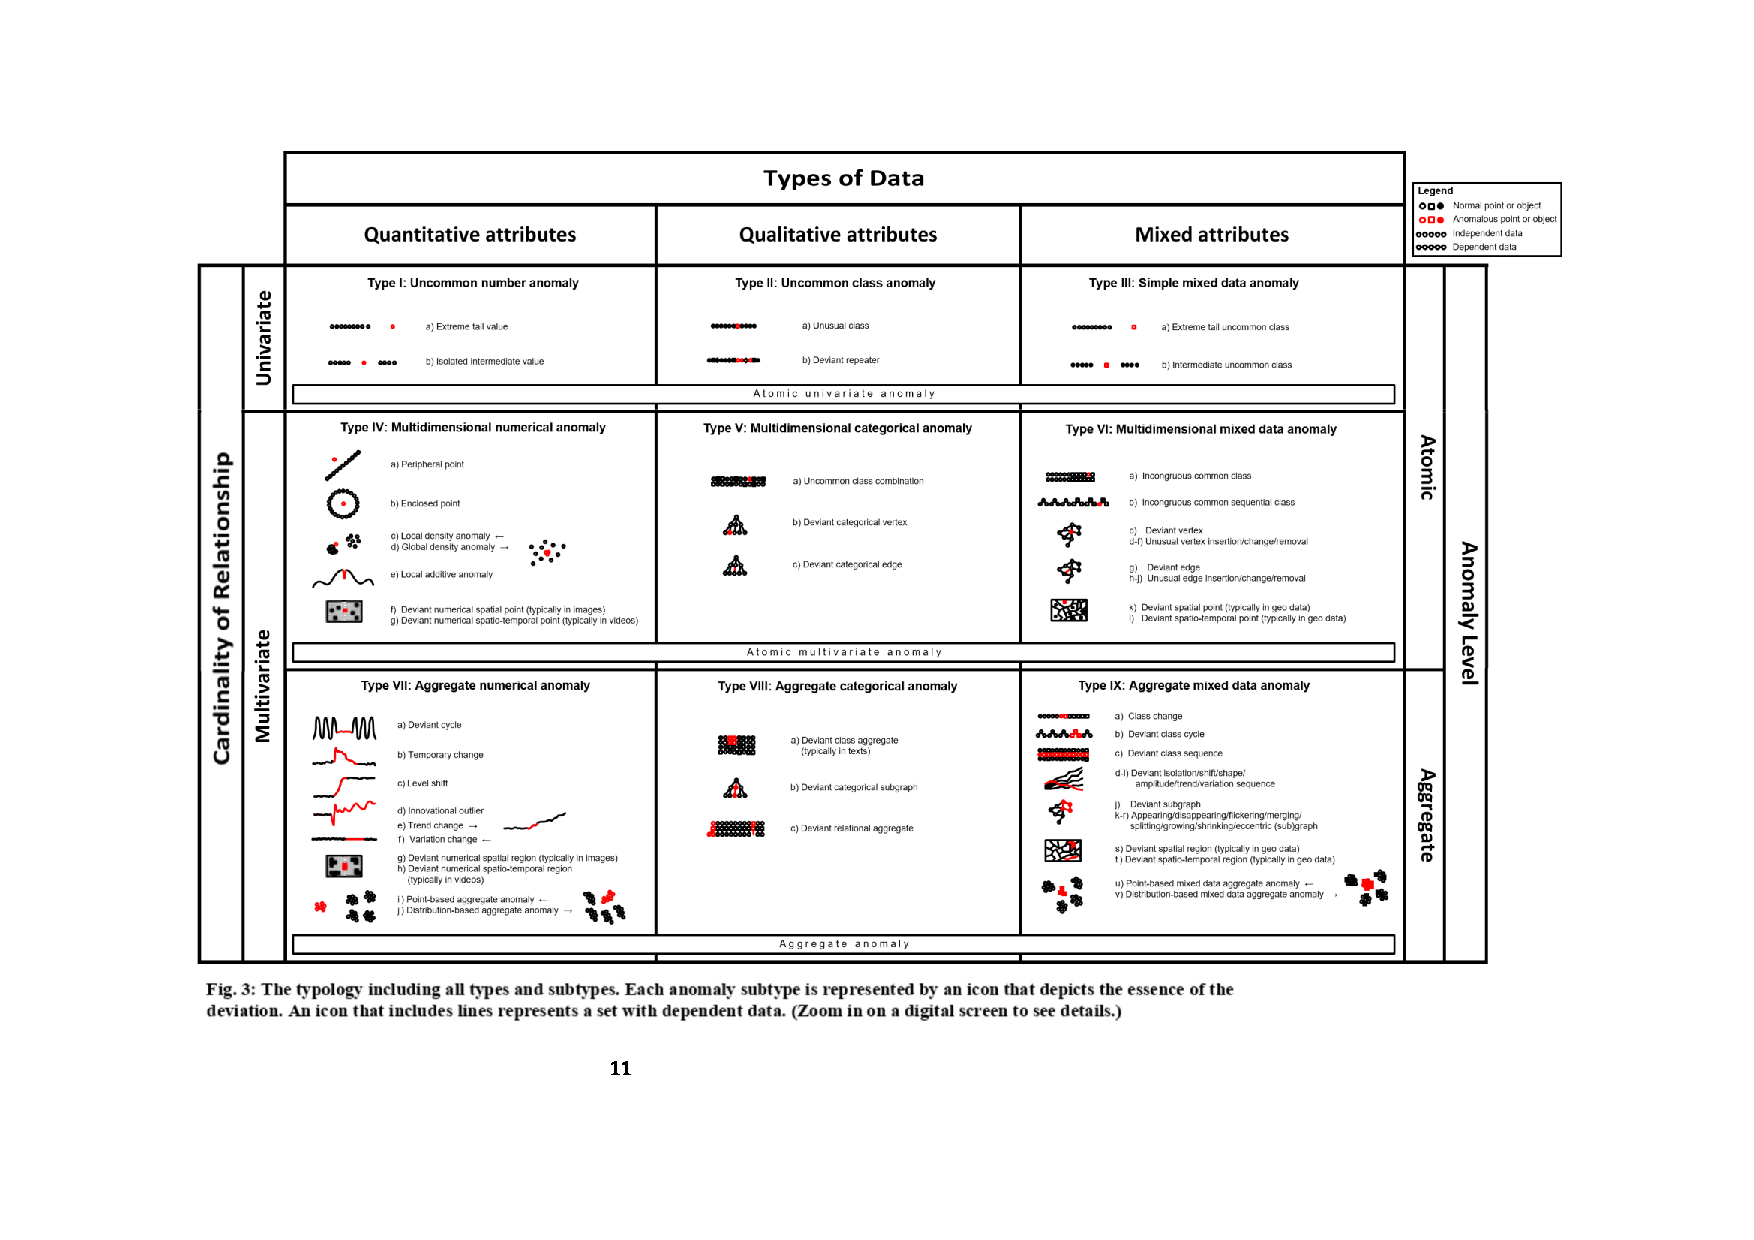
\includegraphics[scale=0.6]{Figures/Anomaly_types_t}
	\decoRule
	\caption[CNN Architecture for Time Series]{CNN Architecture for Time Series \parencite{Munir2019}}
	\label{fig:Anomaly_types}
	%https://ieeexplore.ieee.org/document/8581424?denied=
\end{figure}

\subsection{title}